\documentclass[12pt,a4paper,onecolumn]{article}
\usepackage[utf8]{inputenc}
\usepackage[T1]{fontenc}
\usepackage[french]{babel}

\usepackage{multicol}
\usepackage{fullpage}

% ------------------------- Color table ----------------------------------------
\usepackage{multirow}
\usepackage[table]{xcolor}
\definecolor{maroon}{cmyk}{0,0.87,0.68,0.32}
\usepackage{booktabs} % to make prettier tables (toprule, midrule, bottomrule)
% ------------------------------------------------------------------------------

\usepackage{amscd}
\usepackage{amsthm}
\usepackage{physics}
\usepackage{fullpage}
\usepackage{textcomp,gensymb} %pour le °C, et textcomp pour éviter les warning
\usepackage{graphicx} %pour les images
\usepackage{caption}
\usepackage{subcaption}
\usepackage[colorlinks=true,
	breaklinks=true,
	citecolor=blue,
	linkcolor=blue,
	urlcolor=blue]{hyperref} % pour insérer des liens
\usepackage{epstopdf} %converting to PDF
\usepackage[export]{adjustbox} %for large figures

\usepackage{array}
\usepackage{dsfont}% indicatrice : \mathds{1}


% -------------------------- Mathematics ---------------------------------------
\graphicspath{{images/}{../images/}} % For the images path
% ------------------------------------------------------------------------------

% -------------------------- Mathematics ---------------------------------------
\usepackage{mathrsfs, amsmath, amsfonts, amssymb}
\usepackage{bm}
\usepackage{mathtools}
\usepackage[Symbol]{upgreek} % For pi \uppi different from /pi

% For pseudo-code
\usepackage[ruled,vlined,linesnumbered,noresetcount]{algorithm2e}

\newcommand{\R}{\mathbb{R}} % For Real space
\usepackage{tikz}
\usetikzlibrary{bayesnet} %library to draw graphical models1
% ------------------------------------------------------------------------------


% -------------------------- Code format ---------------------------------------
\usepackage[numbered,framed]{matlab-prettifier}
\lstset{
	style              = Matlab-editor,
	basicstyle         = \mlttfamily,
	escapechar         = '',
	mlshowsectionrules = true,
}
% ------------------------------------------------------------------------------

% ------------------------- Blbiographie --------------------------------------
\usepackage[backend=biber, style=ieee]{biblatex}
\addbibresource{biblio.bib}
\usepackage{csquotes}
% ------------------------------------------------------------------------------


\setcounter{tocdepth}{4} %Count paragraph
\setcounter{secnumdepth}{4} %Count paragraph
\usepackage{float}

\usepackage{graphicx} % for graphicspath
% \graphicspath{{../images/}}

\usepackage{array,tabularx}
\newcolumntype{L}[1]{>{\raggedright\let\newline\\\arraybackslash\hspace{0pt}}m{#1}}
\newcolumntype{C}[1]{>{\centering\let\newline\\\arraybackslash\hspace{0pt}}m{#1}}
\newcolumntype{R}[1]{>{\raggedleft\let\newline\\\arraybackslash\hspace{0pt}}m{#1}}


\usepackage{hyperref}

% \setcounter{section}{5} % to start counting section to 6

% Independent sign
\newcommand{\indep}{\ensuremath{\,\bot\!\!\!\bot\,}} %% The symbol for independent

% Alpha / Numbers for sections
\renewcommand{\thesubsubsection}{\arabic{section}.\arabic{subsection}.\alph{subsubsection})}

% Norm
\newcommand{\norm}[1]{\left\lVert#1\right\rVert}


% ------------------------ General informations --------------------------------
\title{Math M2 Probabilistic graphical models 2017/2018}
\author{Vincent Matthys}
\graphicspath{{images/}}
% http://www.cedar.buffalo.edu/~srihari/CSE574/Chap13/Ch13.2-HiddenMarkovModels.pdf
% https://www.cs.cmu.edu/~epxing/Class/10701-08s/recitation/em-hmm.pdf
% ------------------------------------------------------------------------------



\begin{document}
\begin{tabularx}{0.8\textwidth}{@{} l X r @{} }
	{\textsc{Master MVA}}                   &  & \textsc{Homework 3} \\
	\textsc{Probabilistic graphical models} &  & {Vincent Matthys}   \\
\end{tabularx}
\vspace{1.5cm}
\begin{center}
	\rule[11pt]{5cm}{0.5pt}

	\textbf{\LARGE \textsc{Compte-rendu du devoir 3}}
	\vspace{0.5cm}\\
	Vincent Matthys\\
	\rule{5cm}{0.5pt}
	\vspace{1.5cm}
\end{center}

\section{HMM implementation}



\setcounter{subsection}{-1}
\subsection{Notations}

On désignera par \(M\) le nombre d'états cachés (4 dans notre cas).
On notera \(\bm{u} = \{u_t\}_{t \in [\![1;T]\!]}\), \(\bm{q} = \{q_t\}_{t \in [\![1;T]\!]}\), \(\bm{\theta} = \left(\pi, A, \bm{\mu}, \bm{\Sigma}\right)\) où \(\bm{\mu} = \{\mu_k\}_{k \in [\![1;M]\!]}\) et \(\bm{\Sigma} = \{\Sigma_k\}_{k \in [\![1;M]\!]}\).
On utilisera également le \textit{one-hot encoding} sur \(\bm{q}\), de sorte que \(q_t^i\), variable binaire, représente la i\up{e} composante de \(q_t\).

\subsection{}

Le problème de l'inférence dans la chaine de Markov modélisée, à savoir le calcul de \(p(\bm{q} \mid \bm{u})\) est appréhendable par le calcul de la marginale \(p(q_t \mid \bm{u})\) suivant :

\begin{equation}
	\begin{split}
		p(q_t \mid \bm{u}) &= \frac{p(\bm{u} \mid q_t)p(q_t)}{p(\bm{u})}\\
		&= \frac{p(u_1,\dots,u_t \mid q_t)p(u_{t+1},\dots,u_T \mid q_t) p(q_t)}{p(\bm{u})} \quad u_1,\dots,u_t \indep u_{t+1},\dots,u_T \mid q_t\\
		&= \frac{p(u_1,\dots,u_t, q_t)p(u_{t+1},\dots,u_T \mid q_t)}{p(\bm{u})}\\
		&= \frac{\alpha_t(q_t)\beta_t(q_t)}{p(\bm{u})}\\
		&= \frac{\alpha_t(q_t)\beta_t(q_t)}{\sum_{q_t}\alpha_t(q_t)\beta_t(q_t)}\\
		&= \frac{\alpha_t(q_t)\beta_t(q_t)}{\sum_{q_T}\alpha_T(q_T)} \quad \text{puisque} \quad p(\bm{u}) = \sum_{q_T}p(q_T, \bm{u}) = \sum_{q_T}\alpha_T(q_T)\\
	\end{split}
	\label{filtering_eq}
\end{equation}

avec \(\alpha_t(q_t) = p(u_1,\dots,u_t, q_t)\) et \(\beta_t(q_t) = p(u_{t+1},\dots,u_T \mid q_t)\)

On peut alors aussi exprimer \(p(q_t, q_{t+1} \mid \bm{u})\) en fonction de \(\alpha_t\) et \(\beta_t\) :

\begin{equation}
	\begin{split}
		p(q_t, q_{t+1} \mid \bm{u}) &= \frac{p(\bm{u} \mid q_t, q_{t+1}) p (q_t, q_{t+1})}{p(\bm{u})}\\
		&= \frac{p(\bm{u} \mid q_t, q_{t+1}) p (q_{t+1} \mid q_t) p (q_t)}{p(\bm{u})}\\
		&= \frac{p(u_1, \dots, u_t \mid q_t, q_{t+1}) p(u_{t+1}, \dots, u_T \mid q_t, q_{t+1}) p(q_{t+1} \mid q_t) p (q_t)}{p(\bm{u})}\\
		&= \frac{p(u_1, \dots, u_t \mid q_t) p(u_{t+1}, \dots, u_T \mid q_{t+1}) p(q_{t+1} \mid q_t) p (q_t)}{p(\bm{u})}\\
		&= \frac{p(u_1, \dots, u_t \mid q_t) p(u_{t+1} \mid q_{t+1}) p(u_{t+2}, \dots, u_T \mid q_{t+1}) p(q_{t+1} \mid q_t) p (q_t)}{p(\bm{u})}\\
		&= \frac{p(u_1, \dots, u_t, q_t) p(u_{t+1} \mid q_{t+1}) p(u_{t+2}, \dots, u_T \mid q_{t+1}) p(q_{t+1} \mid q_t)}{p(\bm{u})}\\
		&= \frac{\alpha_t(q_t) p(u_{t+1} \mid q_{t+1}) \beta_t(q_{t+1}) A_{q_t, q_{t+1}}}{p(\bm{u})}\\
	\end{split}
\end{equation}
où \(A_{q_t, q_{t+1}} = p(q_{t+1} \mid q_t)\) et \(p(u_{t+1} \mid q_{t+1})\) suit une loi gaussienne.

À des fins d'implémentation, on considèrera les logarithmes des \(\alpha\) et \(\beta\), \(\tilde{\alpha}\) et \(\tilde{\beta}\) de sorte que les formules de récursion peuvent se réecrire :
\begin{equation}
	\left\{
	\begin{split}
		\ln\alpha_t(q_t) &= \ln p(u_t \mid q_t) + \ln\sum_{q_{t-1}}\left(e^{\ln \alpha_{t-1}(q_{t-1})}A_{q_{t-1}, q_{t}}\right)\\
		\ln\beta_t(q_t) &= \ln\sum_{q_{t+1}}\left(e^{\ln \beta_{t+1}(q_{t+1})}A_{q_{t}, q_{t+1}}p(y_{t+1}\mid q_{t+1})\right)\\
	\end{split}
	\right.
\end{equation}

\begin{equation}
	\left\{
	\begin{split}
		\tilde{\alpha}_t(q_t) &= \ln p(u_t \mid q_t) + \ln\sum_{q_{t-1}}\left(e^{\tilde{\alpha}_{t-1}(q_{t-1})}A_{q_{t-1}, q_{t}}\right)\\
		\tilde{\beta}_t(q_t) &= \ln\sum_{q_{t+1}}\left(e^{\tilde{\beta}_{t+1}(q_{t+1})}A_{q_{t}, q_{t+1}}p(y_{t+1}\mid q_{t+1})\right)\\
	\end{split}
	\right.
\end{equation}

et que la tâche d'inférence dite de \textit{smoothing} en équation~\eqref{filtering_eq} s'écrit :

\begin{equation}
	\begin{split}
		\ln p(q_t \mid \bm{u}) &= \ln\alpha_t(q_t) + \ln\beta_t(q_t) - \ln \sum_{q_T}\alpha_T(q_T)\\
		\ln p(q_t \mid \bm{u}) &= \tilde{\alpha}_t(q_t) + \tilde{\beta}_t(q_t) - \ln \sum_{q_T}e^{\tilde{\alpha}_T(q_T)}\\
	\end{split}
\end{equation}

La tâche d'inférence dite de \textit{filtering} est également ajoutée en normalisant \(\alpha_t\) :
\begin{equation*}
	\alpha_t^{\text{norm}}(q_t) = p(q_t \mid u_1, \dots, u_t) = \frac{\alpha_t(q_t)}{\sum_{q_t}\alpha_t(q_t)}
\end{equation*}
et est disponible par le calcul des \(\alpha^{\text{norm}}\) dans le code fourni.

\subsection{}

\begin{figure}[H]
	\centering
	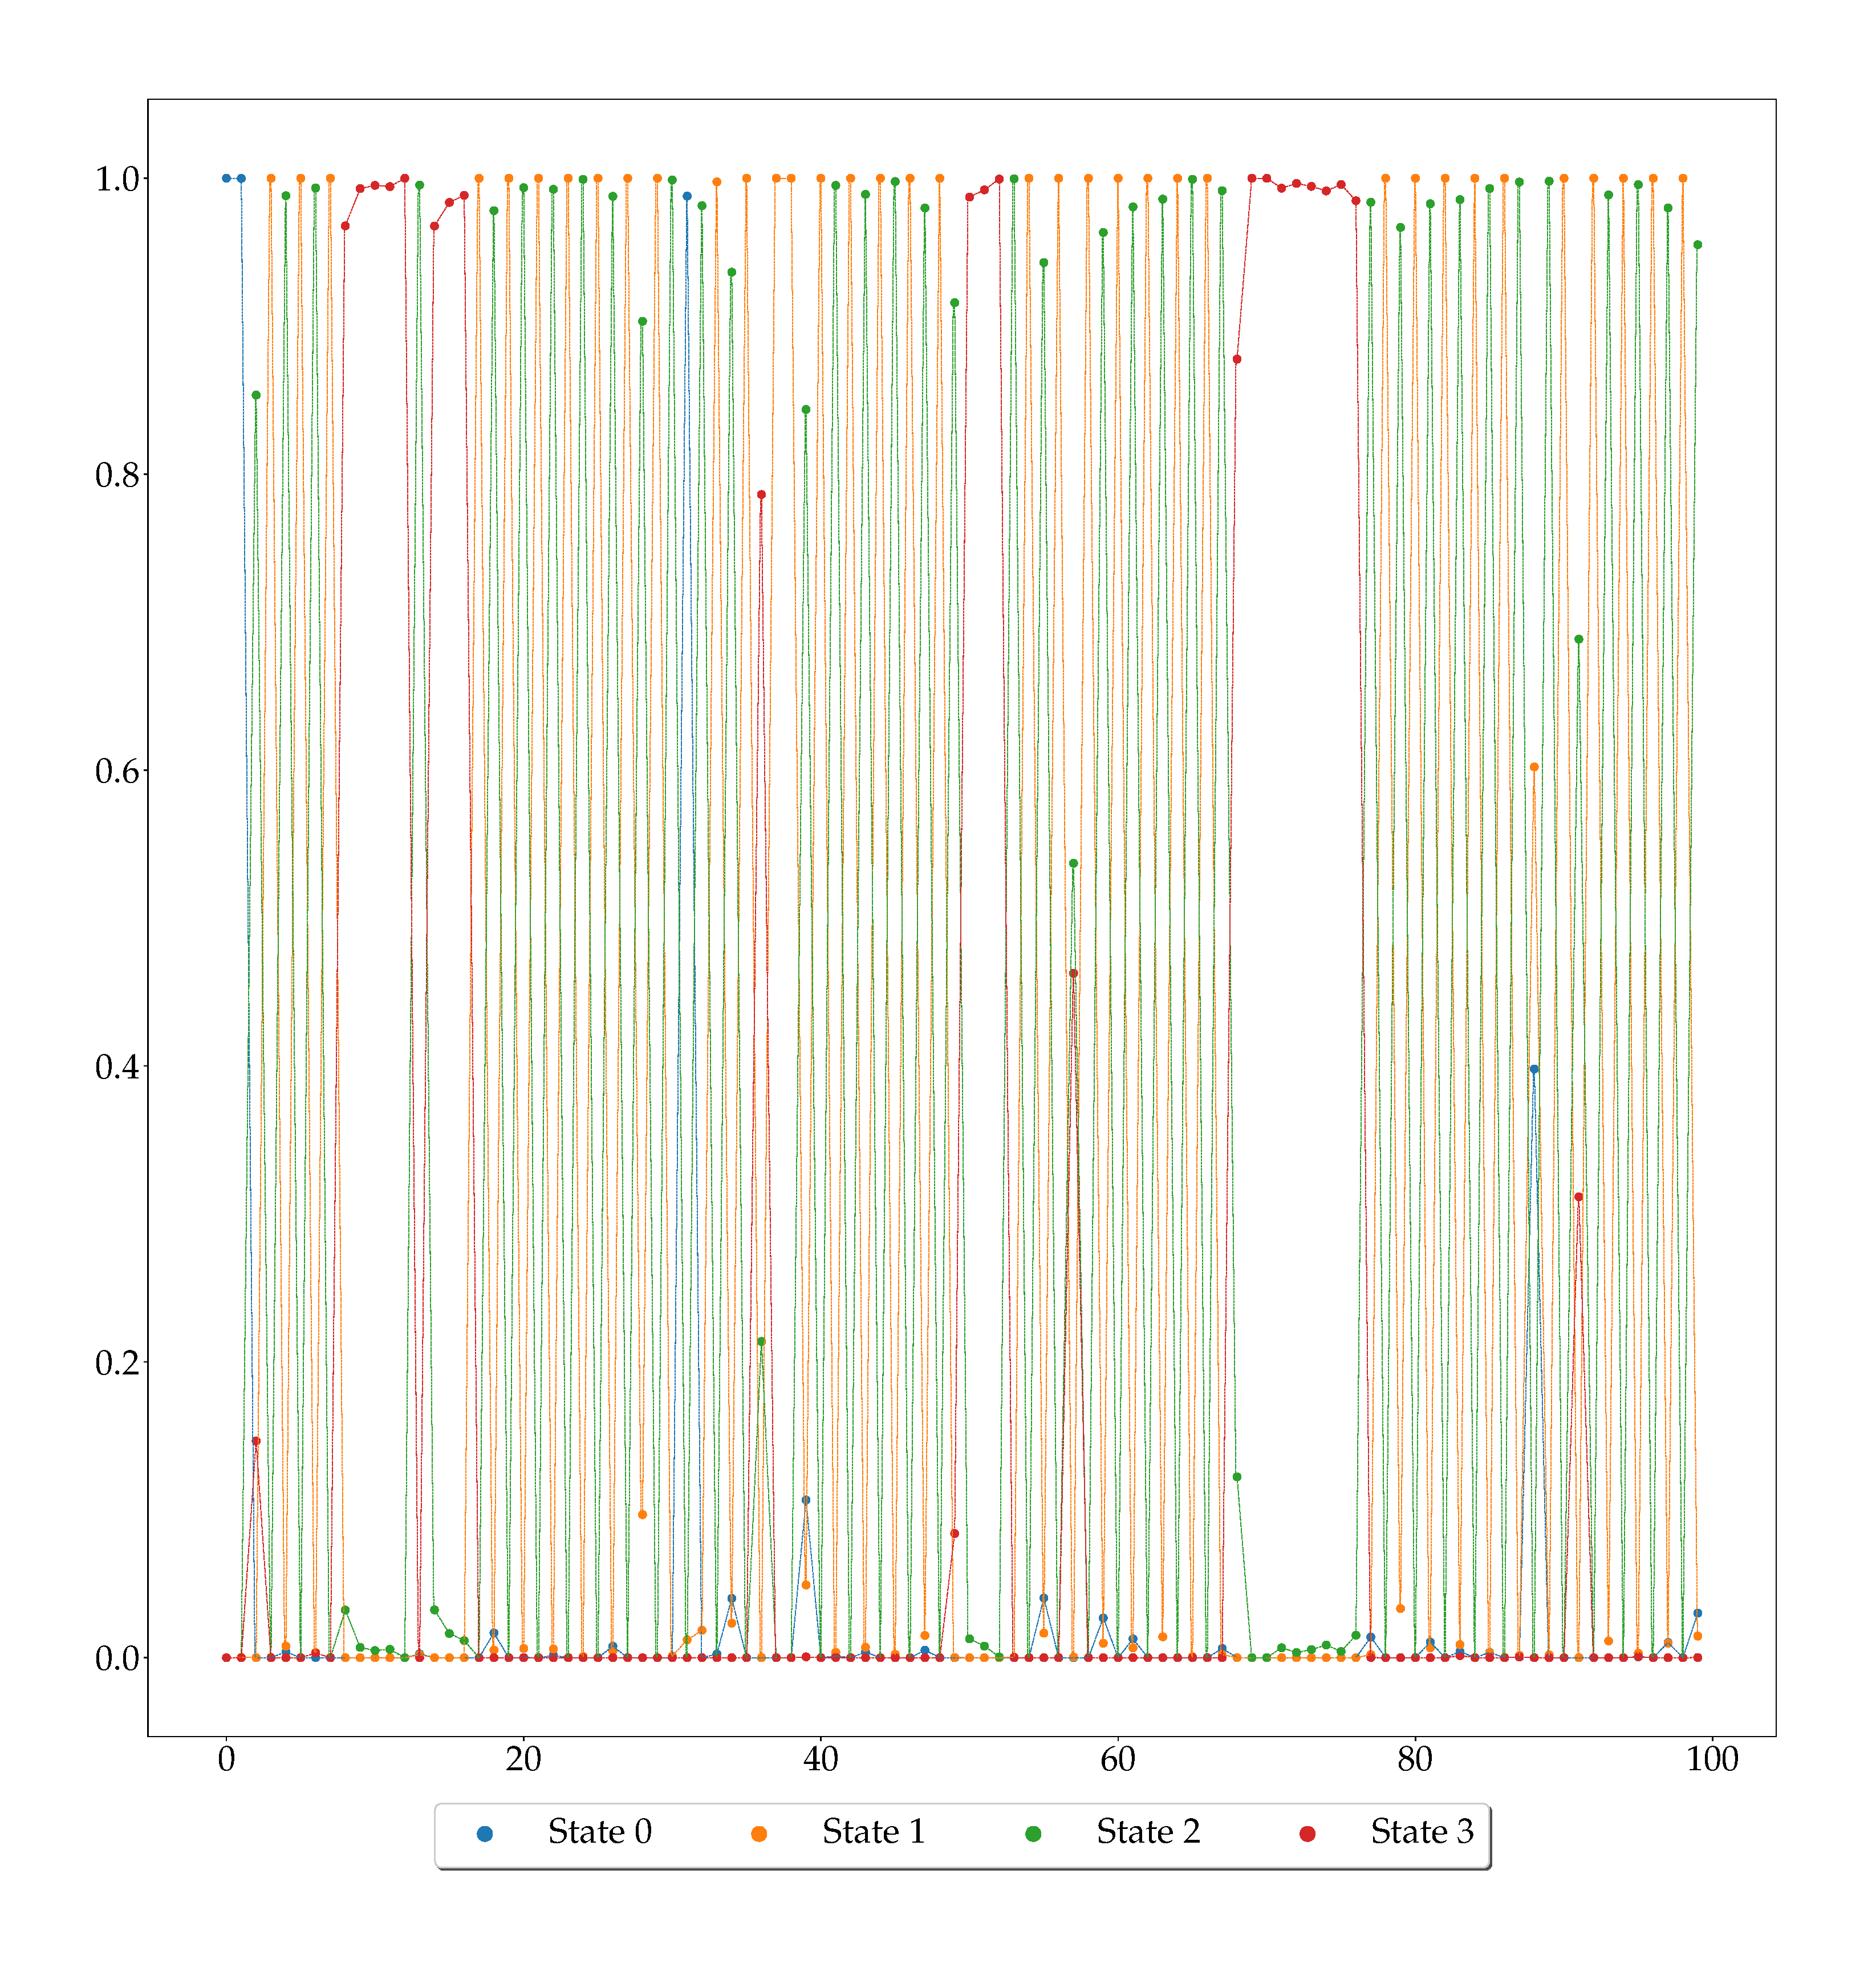
\includegraphics[width = 1.0\textwidth]{2_smoothing.eps}
	\caption{Smoothing result for the first 100 datapoints}
	\label{fig_2_smoothing}
\end{figure}
La figure donnant le résulat du smoothing des 100 premier points est présentée en figure~\ref{fig_2_smoothing}. On y constate notamment une alternance importante entre les états 1 et 2, qui représentent également la majorité des états les plus probables.


\subsection{}

On exprime la log-vraisemblance incomplète de la manière suivante :
\begin{equation}
	\begin{split}
		\ell(\bm{\theta} ; \bm{u}) &= \ln \sum_{\bm{q}}p\left(\bm{q}, \bm{u} \mid \bm{\theta}\right)\\
		&= \ln \sum_{\bm{q}}r(\bm{q} \mid \bm{u}) \frac{p\left(\bm{q}, \bm{u} \mid \bm{\theta}\right)}{r(\bm{q} \mid \bm{u})} \quad \text{pour r quelconque}\\
		&\ge \sum_{\bm{q}}r(\bm{q} \mid \bm{u}) \ln \frac{p\left(\bm{q}, \bm{u} \mid \bm{\theta}\right)}{r(\bm{q} \mid \bm{u})} \quad \text{par l'inégalité de Jensen}\\
		&\ge \mathbb{E}_{r}[\ell_c(\bm{\theta} ; \bm{q}, \bm{u})]- H(r(\bm{q} \mid \bm{u})) = \mathcal{L}(r, \bm{\theta}, \bm{u})\\
	\end{split}
\end{equation}


avec \(\ell_c(\bm{\theta} ; \bm{q}, \bm{u})\), log-vraisemblance complète, dont l'expression est la suivante :
\begin{equation}
	\begin{split}
		\ell_c(\bm{\theta} ; \bm{q}, \bm{u}) &= \ln p\left(\bm{q}, \bm{u} \mid \bm{\theta}\right) \\
		&= \sum_{t=1}^{T}\ln p(u_t \mid q_t, \bm{\mu}, \bm{\Sigma}) + \sum_{t=2}^T \sum_{i = 1}^{M} \sum_{j = 1}^{M} q_{t-1}^i q_t^j \ln A_{ij} + \sum_{i = 1}^M q_1^i \ln \pi_i\\
		&= 	\sum_{t=1}^{T}\sum_{k=1}^M q_t^k \left(-\ln2\pi -\frac{1}{2}\ln|\Sigma_k| - \frac{1}{2}(u_t - \mu_k)^{\intercal}\Sigma_k^{-1}(u_t - \mu_k)\right)\\
		&+ \sum_{t=2}^T \sum_{i = 1}^{M} \sum_{j = 1}^{M} q_{t-1}^i q_t^j \ln A_{ij} + \sum_{i = 1}^M q_1^i \ln \pi_i\\
	\end{split}
	\label{eq_llh_c}
\end{equation}

On a donc une borne inférieure de la log-vraisemblance incomplète, \(\mathcal{L}(r, \bm{\theta}, \bm{u})\). L'algorithme EM consiste en une montée alternée de cette borne inférieure par rapport à \(r\) et \(\bm{\theta}\). En choisissant \(r(\bm{q} \mid \bm{u}) = p(\bm{q} \mid \bm{u}, \bm{\theta})\), on maximise celle-ci, de sorte que les deux étapes de l'algorithme se résument de la manière suivante :
\begin{equation}
	\begin{split}
		E-step \quad r^{(s+1)} &= \operatorname{arg}\max_{r} \mathcal{L}(r, \bm{\theta}^{(s)}, \bm{u}) = p(\bm{q} \mid \bm{u}, \bm{\theta}^{(s)})\\
		M-step \quad \bm{\theta}^{(s+1)} &= \operatorname{arg}\max_{\bm{\theta}} \mathcal{L}(r^{(s+1)}, \bm{\theta}, \bm{u}) = \operatorname{arg}\max_{\bm{\theta}} \mathbb{E}_{r^{(s+1)}}(\ell_c(\bm{\theta} ; \bm{q}, \bm{u}))\\
	\end{split}
	\label{eq_EM_steps}
\end{equation}
où \(s\) dénote le nombre d'itérations de l'algorithme.

D'après l'équation~\eqref{eq_llh_c}, on observe que \(m_{ij} \coloneqq \sum_{t=2}^T q_{t-1}^i q_t^j\) est la statistique exhaustive pour \(A_{ij}\), que \(q_1^i\) est la statistique exhaustive pour \(\pi_i\). Les estimateurs de maximum de log-vraisemblance complète pour \(A\) et \(\pi\) sont donc :

\begin{align}
	\widehat{\pi}_{i} & = q_1^i                              \label{eq_pi_MLE}  \\
	\widehat{A}_{ij}  & = \frac{m_{ij}}{\sum_{k = 1}^M m_{ik}} \label{eq_A_MLE}
\end{align}
D'autre part, grâce aux calculs déjà effectués pour les estimateurs de vraisemblance de la mixture de gaussiennes, on obtient les estimateurs de log-vraisemblance complète des paramètres d'émission :
\begin{align}
	\widehat{\mu_k}    & = \frac{\sum_{t = 1}^T q_{t}^k u_t}{\sum_{t = 1}^T q_{t}^k}                                                     \\
	\widehat{\Sigma_k} & = \frac{\sum_{t = 1}^T q_t^k\left(u_t - \mu_k\right)\left(u_t - \mu_k\right)^{\intercal}}{\sum_{t = 1}^T q_t^k}
\end{align}

Ces estimateurs doivent être pris sous l'espérance précise obtenue lors de l'étape E de l'algorithme EM, donnée par l'équation~\eqref{eq_EM_steps}, afin que la maximisation de la log-vraisemblance complète induise une augmentation de la log-vraisemblance incomplète lors de l'itération \(s + 1\).

En reprenant l'estimateur de \(\pi\) obtenu en équation~\eqref{eq_pi_MLE}, on obtient l'estimateur à l'itération \((s + 1)\) :
\begin{equation}
	\begin{split}
		\widehat{\pi_{i}}^{(s + 1)} &= \mathbb{E}_{\bm{q} \mid \bm{u}, \bm{\theta}^{(s)}}[q_1^i] \\
		&= \mathbb{E}_{q_1 \mid \bm{u}, \bm{\theta}^{(s)}}[q_1^i] \\
		&= p(q_1^i = 1 \mid \bm{u}, \bm{\theta}^{(s)}) \coloneqq \gamma_1^{i, (s+1)}
	\end{split}
\end{equation}

En reprenant l'estimateur de \(A_{ij}\) obtenue en équation~\eqref{eq_A_MLE}, il faut déterminer \(\mathbb{E}_{\bm{q} \mid \bm{u}, \bm{\theta}^{(s)}}[m_{ij}]\). On a :
\begin{equation*}
	\begin{split}
		\mathbb{E}_{\bm{q} \mid \bm{u}, \bm{\theta}^{(s)}}[m_{ij}] &= \sum_{t=2}^T \mathbb{E}_{\bm{q} \mid \bm{u}, \bm{\theta}^{(s)}}\left[q_{t-1}^i q_t^j\right]\\
		&= \sum_{t=2}^T p\left(q_{t-1}^i = 1, q_t^j = 1 \mid \bm{u}, \bm{\theta}^{(s)}\right)\\
		&\coloneqq \sum_{t=2}^T \xi^{ij, (s+1)}_{t-1, t}
	\end{split}
\end{equation*}
D'où l'estimateur à l'itération \((s+1)\) pour \(A\) :
\begin{equation}
	\widehat{A}_{ij}^{(s+1)} = \frac{\sum_{t=2}^T \xi^{ij, (s+1)}_{t-1, t}}{\sum_{k = 1}^M\sum_{t=2}^T \xi^{ik, (s+1)}_{t-1, t}} = \frac{\sum_{t=2}^T \xi^{ij, (s+1)}_{t-1, t}}{\sum_{t=2}^T \gamma^{i, (s+1)}_{t-1}}
\end{equation}

De la même façon, on obtient les estimateurs à l'itération \((s+1)\) pour les \(\mu_k\) et \(\Sigma_k\) :

\begin{equation}
	\begin{aligned}
		\widehat{\mu_k}^{(s+1)}    & = \frac{\sum_{t = 1}^T \gamma_{t}^{k,(s+1)} u_t}{\sum_{t = 1}^T \gamma_{t}^{k,(s+1)}} \quad \forall k \in [\![1;M]\!]                                                                     \\
		\widehat{\Sigma_k}^{(s+1)} & = \frac{\sum_{t = 1}^T \gamma_{t}^{k,(s+1)}\left(u_t - \mu_k^{(s)}\right)\left(u_t - \mu_k^{(s)}\right)^{\intercal}}{\sum_{t = 1}^T \gamma_{t}^{k,(s+1)}} \quad \forall k \in [\![1;M]\!] \\
	\end{aligned}
\end{equation}

L'implémentation du calcul des \(\gamma\) et \(\xi\) est succintement détaillée et fait intervenir le calcul des \(\alpha^{\text{norm}}\) du problème de \textit{filtering}.
\begin{equation}
	\begin{split}
		\gamma_t(q_t) &= p(q_t \mid u_1, \dots, u_T)\\
		&= \sum_{q_{t+1}}p(q_t, q_{t+1} \mid u_1, \dots, u_T)\\
		&= \sum_{q_{t+1}} \frac{\alpha_t(q_t)A_{q_t, q_{t+1}}}{\sum_{q_t}\alpha_t(q_t)A_{q_t, q_{t+1}}}\gamma_{t+1}(q_{t+1})\\
		&= \sum_{q_{t+1}} \frac{{\alpha^{\text{norm}}}_{,t}(q_t)A_{q_t, q_{t+1}}}{\sum_{q_t}{\alpha^{\text{norm}}}_{,t}(q_t)A_{q_t, q_{t+1}}}\gamma_{t+1}(q_{t+1})\\
	\end{split}
\end{equation}

\begin{equation}
	\begin{split}
		\xi_{t,t+1}(q_t, q_{t+1}) &= p(q_t, q_{t+1} \mid \bm{u})\\
		&= \frac{\alpha_t(q_t)p(u_{t+1} \mid q_{t-1})\gamma_{t+1}(q_{t+1})A_{q_t, q_{t+1}}}{\alpha_{t+1}(q_{t+1})}\\
		&= \frac{\alpha^{\text{norm}}_t(q_t)p(u_{t+1} \mid q_{t-1})\gamma_{t+1}(q_{t+1})A_{q_t, q_{t+1}}}{\alpha^{\text{norm}}_t(q_{t+1})} \times \frac{\sum_{q_t}\alpha_t(q_t)}{\sum_{q_{t+1}}\alpha_{t+1}(q_{t+1})}\\
	\end{split}
\end{equation}

Au niveau de l'implémentation, on notera qu'on utilise les \(\alpha^{\text{norm}}\) qui ne changent aucunement la formule pour \(\gamma\). Pour \(\xi\), il faut prendre en compte la différence de normalisation entre les \(\alpha^{\text{norm}}\).


\subsection{}

La partie d'implémentation est effectuée toujours en python dans la classe \textit{HMM}.

\subsection{}

\begin{figure}[H]
	\centering
	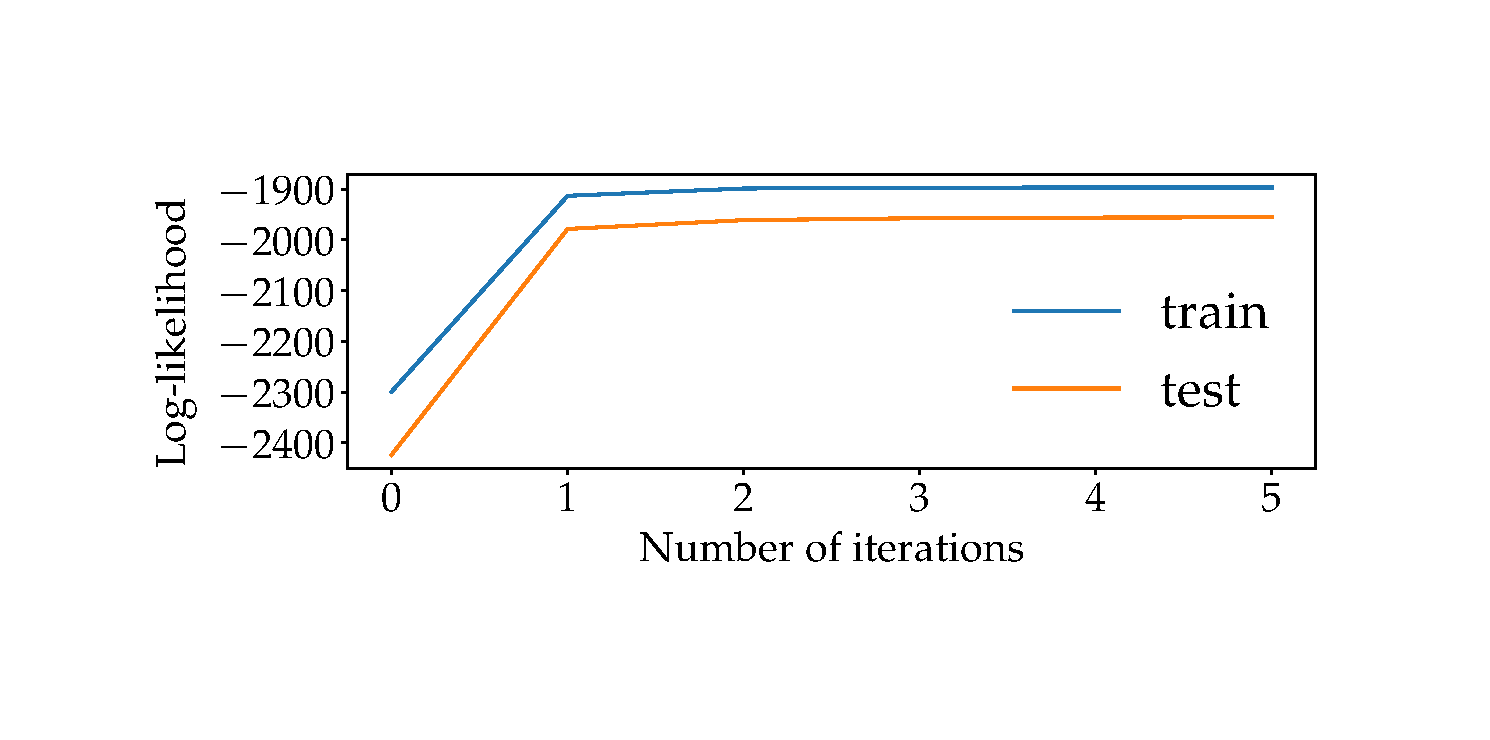
\includegraphics[width = 1.0\textwidth]{5_em_llh}
	\caption{Log-likelihood}
	\label{fig_5_llh_em}
\end{figure}

La log-vraisemblance en apprentissage et en test est représentée en figure~\ref{fig_5_llh_em}. On constate qu'il suffit de 2-3 itérations de l'algorithme EM pour converger vers de nouveaux paramètres, en partant de ceux déterminés par mixture de gaussienne. On constate également que la vraisemblance en apprentissage est toujours supérieure à la vraisemblance de test, ce qui constitue un résultat attendu.



\end{document}
